\documentclass[11pt]{article}
\usepackage[a4paper,margin=24mm]{geometry}
\usepackage{amsmath,amssymb,mathtools,tikz}
\usepackage[hidelinks]{hyperref}\usepackage{xurl}
\usetikzlibrary{arrows.meta}
\setlength{\emergencystretch}{3em}
\newcommand{\C}{\mathbb C}\newcommand{\ip}[2]{\langle#1,#2\rangle_G}
\title{The original adjacent cutoffs:\\determinant allocation and the complete complex current}
\author{Split-Zero research programme}\date{21 September 2026}
\begin{document}\maketitle
Adding the next orthogonal polynomial changes the original attained
quotient covariance by one column. We calculate its effect on the actual
conductor kernel and both complex projected currents. Every coefficient
of the adjacent-cutoff sign polynomial is displayed; its degree is at
most five, independent of dimension. We also prove that the two adjacent
changes of the original conductor projection determinant cost only
\(O_A(q\log(q+2))=o(kq)\). The remaining leading allocation is reduced
to the two specified original endpoints. Its value and the individual
current signs remain to be evaluated.

\section{Original source and one added column}
Use MR1--10 \cite{MR}, on its complete simple-quartet five-orbit domain:
\begin{equation}\tag{ACC1}
\begin{gathered}
k\ge9,\quad k=1\pmod4,\quad q=(k+1)^2,\quad c=k/2,\\
0<\delta<1/2,\quad\gamma>2,\qquad
\lambda_{ab}=c+(2a-k)\delta+i(2b-k)\gamma,\\
\chi(S)=\prod_{a,b=0}^k(S-\lambda_{ab}),\qquad
d\mu(y)=w_h^{*k}(y)\,dy,\quad S=c+iy .
\end{gathered}
\end{equation}
Keep the original divisor \(h\), source mass, units and period.
Let \(p_j(S)\) be its monic orthogonal polynomials, with actual norms
\(\omega_j>0\). The source has finite moments and positive polynomial
Grams by MR3. The literal root-value map is \(V[P]=(P(\lambda_{ab}))\).
In these coordinates \(A=\operatorname{diag}(\lambda_{ab})\).
Keep the full invariant image \(Z=[M_A,S_kZ_k]\), its annihilator frame
\(B=\pi^T\), and \(K=\operatorname{im}B=\ker Z^T\), of dimension
\(m=8k-16\). The map from polynomial coordinates is \(I_K=V^{-1}B\).
The metrics are related by \(G=V^{-*}G^{\rm pol}V^{-1}\);
thus \(B^*GB=I_K^*G^{\rm pol}I_K\), with no change of the source.

For \(N\ge q-1\), set
\begin{equation}\tag{ACC2}
C=\sum_{j=0}^N u_ju_j^*,\qquad
(u_j)_\alpha=p_j(\lambda_\alpha)/\sqrt{\omega_j},\qquad
G=C^{-1},\qquad u=u_{N+1}.
\end{equation}
Interpolation proves \(C>0\). MR9--10 proves that \(G\) is the full
attained minimum over the entire relation ideal. The next covariance
is exactly \(C_{N+1}=C+uu^*\).
Use \(C(t)=C+tuu^*\), \(t\ge0\), to calculate this single column:
\(t=0,1\) are the original adjacent cutoffs. For \(t>0\) this is the
covariance of the source map with columns
\(u_0,\ldots,u_N,\sqrt t\,u_{N+1}\) from its displayed Euclidean
coefficient space. This specifies every intermediate source map.
The finite identities also apply separately to a specified Gamma source;
its orthogonal polynomials are not identified with the arithmetic ones.

\section{The complete allocation and moving projection}
The inverse update is the classical Sherman--Morrison identity
\cite{SM}. Its needed form is proved below, with the original
source attribution retained.
All following inner products are in \(G\), conjugate-linear first.
Define
\begin{equation}\tag{ACC3}
\begin{gathered}
H=B^*GB,\quad P=BH^{-1}B^*G,\quad e=Pu,\quad f=(I-P)u,\\
a=\|e\|_G^2,\quad\beta=\|f\|_G^2,\quad\alpha=a+\beta=\|u\|_G^2,\\
d(t)=1+t\alpha,\quad b(t)=1+t\beta,\quad s(t)=t/b(t).
\end{gathered}
\end{equation}
Multiplication gives \(P^2=P\), \(P^*G=GP\), and image \(K\).
Thus \(e\perp_G f\), proving the energy equality and \(b,d\ge1\).
Multiplication by \(C+tuu^*\) proves
\begin{equation}\tag{ACC4}
G(t)=G-\frac{t}{d(t)}Guu^*G.
\end{equation}
Write \(h_B=B^*Gu\), so \(h_B^*H^{-1}h_B=a\). Direct multiplication gives
\begin{equation}\tag{ACC5}
H(t)=H-\frac{t}{d(t)}h_Bh_B^*,\qquad
H(t)^{-1}=H^{-1}+\frac{t}{b(t)}H^{-1}h_Bh_B^*H^{-1}.
\end{equation}
For invertible \(T\), expansion of \(\det(I+T^{-1}vw^*)\) by columns
has no term with two updated columns, since those columns are
proportional. Its first-order terms sum to \(w^*T^{-1}v\).
This proves \(\det(T+vw^*)/\det T=1+w^*T^{-1}v\), and hence
\begin{equation}\tag{ACC6}
\boxed{\frac{\det H(t)}{\det H}=\frac{1+t\beta}{1+t\alpha},\qquad
\frac{\det G(t)}{\det G}=\frac1{1+t\alpha}.}
\end{equation}
Choose any fixed complement \(J\) to \(B\), and let \(Q(t)\) be
the quotient minimum in its fixed quotient coordinates. It is the
Schur complement of \(H(t)\) in \([B,J]^*G(t)[B,J]\).
Block elimination gives its determinant factorization. The fixed
frame determinant cancels, proving
\begin{equation}\tag{ACC7}
\boxed{\frac{\det Q(t)}{\det Q(0)}=\frac1{1+t\beta},\qquad
-\frac{d}{dt}\log\det H(t)=
\frac{a}{(1+t\alpha)(1+t\beta)}.}
\end{equation}
The kernel loss in one original step is
\(\log((1+\alpha)/(1+\beta))\); the complementary loss is
\(\log(1+\beta)\). Both use the actual projected column.

Substituting ACC4--5 in \(BH(t)^{-1}B^*G(t)\) gives
\begin{equation}\tag{ACC8}
\boxed{P(t)=P-\frac{t}{1+t\beta}e f^*G.}
\end{equation}
Indeed the coefficient of \(e u^*G\) is
\(-t/d-t^2a/(bd)=-t/b\), and the other added term is
\(t e u^*GP/b\). This verifies the formula while retaining
the original moving projection.

\begin{figure}[ht]\centering
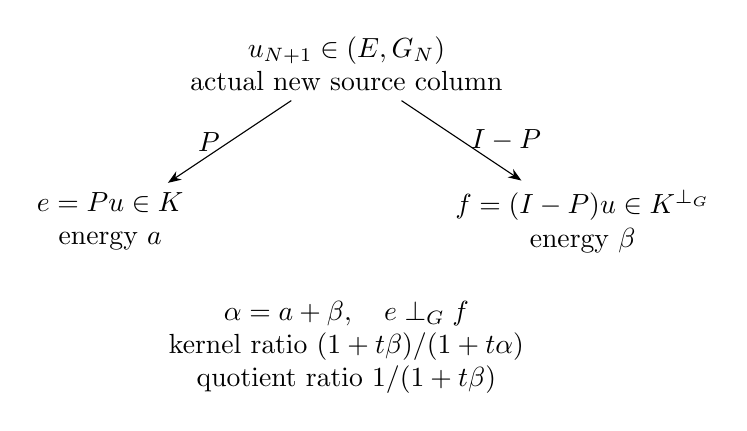
\begin{tikzpicture}[>=Stealth,every node/.style={align=center}]
\node (u) at (0,0) {$u_{N+1}\in(E,G_N)$\\actual new source column};
\node (e) at (-3,-2) {$e=Pu\in K$\\energy \(a\)};
\node (f) at (3,-2) {$f=(I-P)u\in K^{\perp_G}$\\energy \(\beta\)};
\draw[->] (u)--node[left] {\(P\)}(e);
\draw[->] (u)--node[right] {\(I-P\)}(f);
\node at (0,-3.6) {\(\alpha=a+\beta,\quad e\perp_G f\)\\
kernel ratio \((1+t\beta)/(1+t\alpha)\)\\
quotient ratio \(1/(1+t\beta)\)};
\end{tikzpicture}
\caption{Exact maps and energies ACC3--7. The kernel annihilates the
complete original invariant image. No angle or numerical energy is
assigned by the drawing. MR9 supplies the orthogonal-polynomial
source column, with its original human-source citations.}
\end{figure}

\section{Every coefficient of both complex currents}
Fix any original physical class \(x\), without altering its norm.
This includes the actual root eigenclasses. Put
\begin{equation}\tag{ACC9}
p=Px,\quad o=(I-P)x,\quad \rho=f^*Gx=\ip f o,\quad
p_1=\beta p-\rho e,\quad o_1=\beta o+\rho e.
\end{equation}
Then \(P(t)x=(p+tp_1)/b(t)\) and
\((I-P(t))x=(o+to_1)/b(t)\).
Keep the complete arithmetic action in
\begin{equation}\tag{ACC10}
z(t)=\langle P(t)x,A(I-P(t))x\rangle_{G(t)},\qquad
w(t)=\langle(I-P(t))x,AP(t)x\rangle_{G(t)} .
\end{equation}
Define the following actual contractions:
\begin{equation}\tag{ACC11}
\begin{aligned}
J_0&=\ip p{Ao},&
J_1&=\ip{p_1}{Ao}+\ip p{Ao_1},&
J_2&=\ip{p_1}{Ao_1},\\
T_0&=\ip p u\,\ip u{Ao},\\
T_1&=\ip{p_1}u\,\ip u{Ao}+\ip p u\,\ip u{Ao_1},\\
T_2&=\ip{p_1}u\,\ip u{Ao_1}.
\end{aligned}
\end{equation}
All four coefficients of the first numerator are
\begin{equation}\tag{ACC12}
Z_0=J_0,\quad Z_1=J_1+\alpha J_0-T_0,\quad
Z_2=J_2+\alpha J_1-T_1,\quad Z_3=\alpha J_2-T_2 .
\end{equation}
For the second define
\begin{equation}\tag{ACC13}
\begin{gathered}
w_0=\ip o{Ap},\quad
L=\rho\ip o{Ae}+\overline\rho\ip f{Ap},\quad
T_f=|\rho|^2\ip f{Ae},\\
W_0=w_0,\qquad W_1=2\beta w_0-L,\qquad
W_2=\beta^2w_0-\beta L+T_f .
\end{gathered}
\end{equation}
Then the exact complex currents on the whole path are
\begin{equation}\tag{ACC14}
\boxed{z(t)=\frac{\sum_{j=0}^3Z_jt^j}{d(t)b(t)^2},\qquad
w(t)=\frac{\sum_{j=0}^2W_jt^j}{b(t)^2}.}
\end{equation}
To prove this, substitute ACC4 and ACC9 into the first current.
Its numerator is
\(d\ip{p+tp_1}{A(o+to_1)}
-t\ip{p+tp_1}u\ip u{A(o+to_1)}\), which expands to ACC12.
For the second, use \(o+s\rho e\) and \(p-s\rho e\).
Their metric correction contains
\(\langle o+s\rho e,u\rangle_G
=\overline\rho(1+sa)=\overline\rho\,d/b\).
Combining it with the four uncorrected pairing terms gives
\(w=w_0-sL+s^2T_f\). Multiplication by \(b^2\) proves ACC13--14.

The following six real numbers retain all complex phases:
\begin{equation}\tag{ACC15}
\begin{aligned}
r_0&=\Re(\overline Z_0W_0),\\
r_1&=\Re(\overline Z_0W_1+\overline Z_1W_0),\\
r_2&=\Re(\overline Z_0W_2+\overline Z_1W_1+\overline Z_2W_0),\\
r_3&=\Re(\overline Z_1W_2+\overline Z_2W_1+\overline Z_3W_0),\\
r_4&=\Re(\overline Z_2W_2+\overline Z_3W_1),\\
r_5&=\Re(\overline Z_3W_2).
\end{aligned}
\end{equation}
Consequently
\begin{equation}\tag{ACC16}
\boxed{\Re(\overline{z(t)}w(t))
=\frac{\sum_{j=0}^5r_jt^j}{(1+t\alpha)(1+t\beta)^4}.}
\end{equation}
The old endpoint equals \(r_0\); the new endpoint equals
\(\sum_jr_j/((1+\alpha)(1+\beta)^4)\).
A nonzero numerator has at most five positive zeros counted with
multiplicity. If all six coefficients vanish, the current is zero
on the whole path. This covers every degenerate case.
In particular \(f=0\) gives \(\beta=\rho=0\), a constant \(w\) and
a linear numerator for \(z\). If \(u=0\), everything is unchanged.
The finite coefficients specialize the earlier full-current formulas
to the actual source step. Their values still depend on the original
period, class and arithmetic metric; no sign is inferred from volume
monotonicity or from replacing that metric by Gamma.

\section{The adjacent changes of the original projection determinant}
Use the separate lower Gamma source of CGR and CGS \cite{CGR,CGS},
with their exact \(v,c',q',g\) and the same invariant row frame
\(R_Z>0\) at all four cutoffs. Put
\(D=N-v\), \(M=D-q'\), and \(I_N=\chi'\mathcal P'_M\subset\mathcal P'_D\).
The fixed functional for a row \(z\) is
\(\ell_z[P]=[P(\partial_w)G_z(w)]_{w=0}\), with \(G_z=F_z/E_A\).
Polynomial evaluation here uses the original \(S'\) coordinate.
Let \(C_N^U\) be the Gram of these functionals restricted to \(I_N\),
and \(\widetilde C_N\) their Gram on \(\mathcal P'_D\).
Then \(S_N=\widetilde C_N^{-1/2}C_N^U\widetilde C_N^{-1/2}>0\).

There is exactly one orthogonal new direction in each nested
inclusion \(I_N\subset I_{N+1}\), \(\mathcal P'_D\subset\mathcal P'_{D+1}\).
To specify it, form the monic degree-\(M+1\) orthogonal polynomial
\(\psi_{M+1}\) for
\(|\chi'(c'+iy)|^2d\sigma(y)\) on \(S'=c'+iy\), with norm
\(\nu_{M+1}\). All its moments are finite and its Gram is positive.
Then \(\chi'\psi_{M+1}/\sqrt{\nu_{M+1}}\) is the unit complement to
\(I_N\). Let \(\phi_{D+1,c'}\) be the original unit Gamma polynomial.
Define
\(a_N=(\ell_z[\chi'\psi_{M+1}]/\sqrt{\nu_{M+1}})_z\) and
\(b_N=(\ell_z[\phi_{D+1,c'}])_z\).
The two orthogonal decompositions give exactly
\begin{equation}\tag{ACC17}
C_{N+1}^U=C_N^U+a_Na_N^*,\qquad
\widetilde C_{N+1}=\widetilde C_N+b_Nb_N^* .
\end{equation}
These are the same fixed functionals on nested full lower-root ideals.
The determinant identity proved above gives
\begin{equation}\tag{ACC18}
\log\det S_{N+1}-\log\det S_N
=\log(1+a_N^*(C_N^U)^{-1}a_N)
-\log(1+b_N^*\widetilde C_N^{-1}b_N).
\end{equation}
Use the complete finite bounds CGR15 and CGS14--15:
\begin{equation}\tag{ACC19}
\begin{gathered}
l_NR_Z\preceq C_N^U\preceq u_NR_Z,\qquad
\widetilde l_NR_Z\preceq\widetilde C_N\preceq u_NR_Z,\\
l_N=(M_D^2B_{\rm val}qC_A^{2q'})^{-1},\quad
\widetilde l_N=(M_D^2B_E)^{-1},\quad
u_N=V_NM_D^{2D}e^{2J_D}.
\end{gathered}
\end{equation}
The constants are those defined and proved in those complete sources.
Every logarithmic allowance is \(O_A(q\log(q+2))\).
If \(C'=C+aa^*\), all eigenvalues of \(C^{-1/2}C'C^{-1/2}\)
are one except \(1+a^*C^{-1}a\). The bounds \(C\succeq lR\),
\(C'\preceq uR\) imply that last eigenvalue is at most \(u/l\).
Thus, with \(\log^+s=\max(0,\log s)\),
\begin{equation}\tag{ACC20}
\begin{gathered}
0\le\log(1+a_N^*(C_N^U)^{-1}a_N)\le A_N:=\log^+(u_{N+1}/l_N),\\
0\le\log(1+b_N^*\widetilde C_N^{-1}b_N)
\le B_N:=\log^+(u_{N+1}/\widetilde l_N),\\
-B_N\le\delta_N:=\log\det S_{N+1}-\log\det S_N\le A_N .
\end{gathered}
\end{equation}
There is no full-row-rank multiplier: only one eigenvalue changes.
Keeping all four signs proves
\begin{equation}\tag{ACC21}
\begin{aligned}
&\log\frac{\det S_{q-1}\det S_q}{\det S_{2q-1}\det S_{2q}}
=2\log\frac{\det S_{q-1}}{\det S_{2q-1}}
+\delta_{q-1}-\delta_{2q-1},\\
&|\delta_{q-1}-\delta_{2q-1}|
\le E_{\rm adj}:=\max(A_{q-1},B_{q-1})
+\max(A_{2q-1},B_{2q-1})=o_A(kq).
\end{aligned}
\end{equation}
The two adjacent endpoints are retained in the exact correction.

With the full finite error \(E_{\rm DCR}\) of DCR26 \cite{DCR},
\(g=16k-48-v\), and
\(\mathcal Rf=f_{q-1}+f_q-f_{2q-1}-f_{2q}\), this yields
\begin{equation}\tag{ACC22}
\boxed{\left|\mathcal R\log\det H_{K,N}^{\rm ar}
-gq\mathfrak C_\partial
-2\log\frac{\det S_{q-1}}{\det S_{2q-1}}\right|
\le E_{\rm DCR}+E_{\rm adj}=o_{A,h}(kq).}
\end{equation}
For \(k\ge17\), CGP24--27 \cite{CGP} gives the two finite sampled
ratios \(\mathcal A_N^{[T]}\), on its actual pole-canceling rows,
with errors \(P_N+2t_k\log(4/3)\).
Substitution only at these two endpoints proves
\begin{equation}\tag{ACC23}
\begin{aligned}
&\left|\mathcal R\log\det S_N
-2(\mathcal A_{q-1}^{[T]}-\mathcal A_{2q-1}^{[T]})\right|\\
&\quad\le E_{\rm adj}+2(P_{q-1}+P_{2q-1})+8t_k\log(4/3)=o_A(kq).
\end{aligned}
\end{equation}
The sample counts and complementary row costs remain the explicit
CGP20/27 constants. No sampled value or leading coefficient is
presumed computed.

\section{The new activated source: both added columns and their interference}
The new supplied activation proof \cite{Activation}, A28--30, uses the
same fixed tensor section \(Y\) at every cutoff. We verify its exact
receiver here. The scalar source inclusion \(X_N\subset X_{N+1}\)
adds its orthonormal polynomial \(\phi_{N+1}\).
The joint inclusion \(X_N+Y\subset X_{N+1}+Y\) adds the orthogonal
residual \(z=(I-P_{X_N+Y})\phi_{N+1}\). If it is nonzero, divide it
by its physical norm; if it is zero the new column is zero.
Let \(f_N,g_N\) be their respective values in the original quotient.
Every vector of zero value is still part of the physical minimum.
The orthogonal decompositions give, at fixed \(0\le\eta\le1\),
\begin{equation}\tag{ACC24}
C_{N+1}(\eta)=C_N(\eta)+UU^*,\quad
U=[\,\sqrt{1-\eta}\,f_N,\ \sqrt\eta\,g_N\,],\quad
C_N(\eta)=(1-\eta)G_N^{-1}+\eta(G_N^J)^{-1}.
\end{equation}
The symbol \(\eta\) in this section means the source activation only.

The following calculation also covers zero or dependent columns.
Use \(G=C_N(\eta)^{-1}\) and its full original kernel projection \(P\).
For \(U\) having \(d_s\) columns (\(d_s=2\) in ACC24), set
\[
E=PU,\quad F=(I-P)U,\quad
\mathsf A=U^*GU,\quad\mathsf B=F^*GF,\quad
D(t)=I+t\mathsf A,\quad B(t)=I+t\mathsf B.
\]
Both small matrices are positive definite for \(t\ge0\).
Their determinants are denoted \(d(t)\) and \(b(t)\). Direct
multiplication verifies
\begin{equation}\tag{ACC25}
G(t)=G-tGU D(t)^{-1}U^*G,\qquad
P(t)=P-tE B(t)^{-1}F^*G.
\end{equation}
For completeness, put \(H=B_K^*GB_K\) for any fixed kernel frame,
and \(L=B_K^*GU\). Then \(L^*H^{-1}L=E^*GE=\mathsf A-\mathsf B\).
Multiplication proves
\(H(t)^{-1}=H^{-1}+tH^{-1}L B(t)^{-1}L^*H^{-1}\);
substituting it into the kernel projection gives ACC25.
Block elimination of
\(\left(\begin{smallmatrix}I&X\\-Y&I\end{smallmatrix}\right)\)
in either order gives \(\det(I+XY)=\det(I+YX)\).
This proves the exact determinant allocations
\begin{equation}\tag{ACC26}
\frac{\det H(t)}{\det H}=\frac{b(t)}{d(t)},\qquad
\frac{\det Q(t)}{\det Q(0)}=\frac1{b(t)}.
\end{equation}
For the actual two columns,
\begin{equation}\tag{ACC27}
\begin{aligned}
d(t)&=1+t\,\operatorname{Tr}\mathsf A
+t^2(\mathsf A_{11}\mathsf A_{22}-|\mathsf A_{12}|^2),\\
b(t)&=1+t\,\operatorname{Tr}\mathsf B
+t^2(\mathsf B_{11}\mathsf B_{22}-|\mathsf B_{12}|^2).
\end{aligned}
\end{equation}
Both complex interference terms remain. In particular the full
activated kernel loss is exactly \(\log d(1)-\log b(1)\).

There is also an explicit finite polynomial for its original current.
For the unchanged physical class \(x\), put \(p=Px\), \(o=(I-P)x\),
\(\rho=F^*Gx\), and
\[
\Delta(t)=\operatorname{adj}D(t),\quad
\mathcal B(t)=\operatorname{adj}B(t),\quad
v(t)=b(t)p-tE\mathcal B(t)\rho,\quad
w_s(t)=b(t)o+tE\mathcal B(t)\rho .
\]
Define the two scalar polynomials
\begin{equation}\tag{ACC28}
\begin{aligned}
Z(t)&=v(t)^*[d(t)G-tGU\Delta(t)U^*G]A w_s(t),\\
W(t)&=[b(t)o^*G-t\rho^*\mathcal B(t)F^*G]A v(t).
\end{aligned}
\end{equation}
Conjugation here acts on coefficients with real \(t\).
Then the two currents ACC10 satisfy exactly
\begin{equation}\tag{ACC29}
z(t)=\frac{Z(t)}{d(t)b(t)^2},\qquad
w(t)=\frac{W(t)}{b(t)^2},\qquad
\Re(\overline zw)=\frac{\Re(\overline{Z(t)}W(t))}{d(t)b(t)^4}.
\end{equation}
To check the cancellation in the second formula, write
\(o_t=o+tEB(t)^{-1}\rho\).
Since \(U^*Go_t=D(t)B(t)^{-1}\rho\), ACC25 gives
\(o_t^*G(t)=o^*G-t\rho^*B(t)^{-1}F^*G\).
The first formula is direct substitution. Thus every factor and
both moving projections are accounted for.

The adjugates have degree at most \(d_s-1\).
Hence \(v,w_s\) have degree at most \(d_s\), the bracket defining
\(Z\) has degree at most \(d_s\), and
\[
\deg Z\le3d_s,\quad \deg W\le2d_s,\quad
\deg\Re(\overline ZW)\le5d_s.
\]
For the new activated adjacent cutoffs this is degree at most ten.
Its endpoint is obtained by \(t=1\) in ACC28--29, with exactly
the original \(U\) of ACC24. This supplies the missing fixed-kernel
and complex-current receivers of the two-column covariance
calculation. It does not assign those native phases from its
\(q^2\) determinant coefficient.

\begin{thebibliography}{9}
\bibitem{SM} J. Sherman and W. J. Morrison,
\emph{Adjustment of an Inverse Matrix Corresponding to a Change
in One Element of a Given Matrix}, Annals of Mathematical Statistics
21 (1950), 124--127,
\href{https://doi.org/10.1214/aoms/1177729893}{doi:10.1214/aoms/1177729893}.
\bibitem{Activation} Supplied web-session derivation,
\emph{The actual outgoing polynomial under source activation},
A1--38, received 21 September 2026. The complete source is retained
with this continuation; human authorship is unspecified in that source.
\bibitem{MR} Split-Zero research programme,
\emph{The original observation kernel as an exact mixed-relation
determinant}, MR1--10.
\href{https://github.com/KokunoYumeto/zeta-function-research-reader/blob/5992ad50c0f2a06921f1fcaded7b4e38097c0739/workbenches/splitzero-tandem/continuations/20260920-original-kernel-mixed-determinants/ORIGINAL_KERNEL_MIXED_DETERMINANT.tex#L36}{Complete pinned public proof}.
\bibitem{CGR} Split-Zero research programme,
\emph{The original covariance and its conductor-pole filtration},
CGR13--17, complete source supplied with this continuation.
\bibitem{CGS} Split-Zero research programme,
\emph{The original strip and its projection-angle loss},
CGS13--22, complete source supplied with this continuation.
\bibitem{DCR} Split-Zero research programme,
\emph{The evaluated outer return and the actual arithmetic kernel},
DCR1--27, especially DCR26, complete source supplied with this continuation.
\bibitem{CGP} Split-Zero research programme,
\emph{The original lower-root projection: exact action, zero kernel,
and a finite determinant formula with \(o(kq)\) error},
CGP1--28, reproduced completely in the reader.
\bibitem{DLMF} T. H. Koornwinder, R. Wong, R. Koekoek,
R. F. Swarttouw, with W. P. Reinhardt,
\emph{Orthogonal Polynomials}, Chapter 18 of the
NIST Digital Library of Mathematical Functions,
F. W. J. Olver et al., editors,
\url{https://dlmf.nist.gov/18.22.E8} and
\url{https://dlmf.nist.gov/18.23.E7}.
The original-author TeX recurrence and generating-function encodings
are retained in the source ledger. Their exact Gamma specialization is
proved in the accompanying CG and CGP sources. Every inverse, projection,
determinant and current identity needed above is proved directly here.
\end{thebibliography}\end{document}
